\chapter{Návrh}
\phantomsection

\section{Požiadavky na aplikáciu a existujúce riešenia}
%TODO api cisco verzie problemy
Kľúčovou vlastnosťou je modularita navrhovanej aplikácie, vďaka ktorej bude možné pridávať a definovať nové moduly na odhaľovanie a opravu nedostatkov alebo meniť existujúce pri zmene syntaxe a sémantike príkazov. Modularita taktiež umožňuje vytvorenie a podporu ďalších výrobcov a operačných systémov sieťových zariadení. Existujúce riešenia sú zväčša zamerané iba na jedného výrobcu a operačný systém, pričom program je jeden zdrojový súbor, ktorý bez dobrej znalosti kódu je problematické upraviť a rozšíriť. Preto jednotlivé overovania odporúčaní a ich následná oprava bude každé v~separátnom module, ktorý budú musieť dodržať určité vstupy a výstupy, teda akési \zkratka{zkAPI}. Existujúce riešenia nedisponujú žiadnym generovaním opravnej konfigurácie na základe nálezu nedostatku, preto  vzniknutá aplikácia bude podporovať aj vygenerovanie nápravy.

Príkladom open-source riešenia je \texttt{Cisco Config Analysis Tool} \cite{AU81CvNW4q8RGnqM}, ktorý čerpá odporúčania z~jednej z~kníh \cite{Singh2018}, pomocou ktorej boli vytvorené aj odporúčania v~tejto práci. V~tomto riešení však chýba veľa dôležitých prevádzkových a bezpečnostných odporúčaní z~dôvodu, že námetom na kontrolný zoznam pri zostavovaní aplikácie bola iba jedna kniha. Taktiež podporuje iba jedného výrobcu sieťových zariadení a chýba mu modularita, nerozlišuje odporúčania a kontrolu ich prítomnosti na základe umiestnenia sieťového zariadenia v~hierarchickom modeli. Existujúci nástroj \texttt{Cisco Config Analysis Tool} obsahuje kontrolu iba na niektoré bezpečnostné nastavenie pre protokol IPv6. Nástrojom s~podobnými vlastnosťami a nedostatkami je aj \texttt{Router Auditing Tool} \cite{OniomAfGpef53LHq}, ktorý má naviac aj \zkratka{zkGUI}. Existuje niekoľko rozšírení aj pre nástroj \texttt{Nessus}, ktoré overujú dodržiavanie odporúčaní a podľa zistení čerpajú z~CIS Benchmarku \cite{CIS_DrTLsgXv24lxeIIM} prípadne z~ekvivalentu benchmarku pre zariadenia od výrobcu Juniper. Taktiež však nepodporujú zjednanie nápravy a ignorujú umiestnenie zariadenia v~topológii.     

Výhodou výsledného programu je aj, že kontrolný zoznam vznikol z~viacerých knižných odporúčaní a benchmarkov organizácií zaoberajúcimi sa danou problematikou. Program bude umožňovať spúšťanie modulov zodpovedných za nájdenie a odstránenie nedostatkov na základe definovaného umiestnenia zariadenia v~hierarchickom modely siete. Tým sa zamedzí generovaniu falošne pozitívnych správ, ktoré by vznikli v~dôsledku overovania nerelevantných požiadavkov na zariadenie v~danej vrstve modelu. V~neposlednom rade bude riešenie zdarma s~možnosťou nahliadnuť a modifikovať respektíve rozšíriť kód. Program bude umožňovať kontrolu odporúčaní aj pre protokol IPv6, ktorým sa príliš nezaoberá väčšina odporúčaní a benchmarkov.

\newpage
\noindent
\\
Kľúčové vlastnosti:

\begin{itemize}
	\item Modularita\,--\,každé overenie a náprava bude v~zvlášť súbore prihliadajúc na na výrobcu a operačný systém pre ktoré je určené.
	\vspace{0.5em}
	\item Prispôsobenie na ďalších výrobcov\,--\,definovanie API pre moduly na budúcu podporu pre zariadenia od viacerých výrobcov a ich operačných systémov.
	\vspace{0.5em}
	\item Zjednanie nápravy\,--\,pri nájdení nedostatku vygenerovanie opravného nastavenia.
	\vspace{0.5em}
	\item Podpora IPv6\,--\,detekcia zlého alebo chýbajúceho nastavenia a následná náprava pre protokol IPv6.
	\vspace{0.5em}
	\item Hierarchický model\,--\,skenovanie nedostatkov typických pre jednotlivé vrstvy, v~ktorých sa zariadenia nachádzajú a tým zníženie falošne pozitívnych varovaní.\vspace{0.5em}
	\item Definuje závažnosti\,--\,každý nájdený nedostatok je hodnotený na 4 stupňovej škále.
	\vspace{0.5em}
	\item Personalizácia\,--\,definovanie modulov, ktoré sa spustia pre jednotlivé vrstvy, zmena závažnosti nájdených nedostatkov v~konfiguračných súboroch
	\vspace{0.5em}
	\item Zoznam útokov a problémov verzie operačného systému
	\vspace{0.5em}
	\item Vygenerovanie správy s~nedostatkami
\end{itemize}

\newpage
\section{Rozdelenie príkazov}
Na zariadeniach od firmy Cisco s~operačným systémom IOS bol vykonaný rozbor možných príkazov a ich foriem zápisu a početnosti výskytu v~konfigurácií. Tento rozbor bol spravený z~dôvodu, že niektoré príkazy sa môžu opakovať a zároveň jeden druh príkazu môže byť konfigurovaný v~rôznych kontextoch a teda neprítomnosť v~jednom kontexte automaticky neznamená nedostatok v~konfigurácií. Na základe rozboru boli rozdelené príkazy na konfiguráciu sieťových zariadení do nasledujúcich štyroch kategórií:
\\
\begin{enumerate}
	\item Maximálne s~jedným výskytom v~konfigurácii\,--\,príkladom môže byť verzia protokolu \zk{zkSSH}.
	
\begin{minipage}{\linewidth}		
\begin{lstlisting}[frame=single,numbers=right,caption={Konfigurácia verzie protokolu SSH},label=lst:ver-ssh,basicstyle=\ttfamily\small, keywordstyle=\color{black}\bfseries\underbar,language=,]
Router(config)#ssh version 2
\end{lstlisting}
\end{minipage}
	
	\item \vspace{2em} Viacnásobný výskyt viazaný na rozhranie\,--\,typickým príkladom je zabezpečenie portu s~definovaním maximálneho počtu povolených \zkratka{zkMAC} adries.
	
\begin{minipage}{\linewidth}		
\begin{lstlisting}[frame=single,numbers=right,caption={Konfigurácia maximálneho počtu povolených MAC adries na porte},label=lst:mac-max,basicstyle=\ttfamily\small, keywordstyle=\color{black}\bfseries\underbar,language=,breaklines=true]
Router(config)#interface FastEthernet0/1
Router(config-if)#switchport port-security mac address maximum 1
\end{lstlisting}
\end{minipage}

	\item \vspace{2em} Viacnásobný výskyt v~konfigurácii\,--\,tieto príkazy konfigurujú rôzne služby, napríklad autentifikáciu správ \zkratka{zkOSPF}.

\begin{minipage}{\linewidth}		
\begin{lstlisting}[frame=single,numbers=right,caption={Konfigurácia autentizácie OSPF na porte alebo v~proccese},label=lst:ospf-auth,basicstyle=\ttfamily\small, keywordstyle=\color{black}\bfseries\underbar,language=,breaklines=true]
Router(config)#interface FastEthernet0/1
Router(config-if)#ip ospf message-digest-key 1 md5 heslo
Router(config-if)#ip ospf authentication message-digest
Router(config)#router ospf 1
Router(config)#area 0 authentication message-digest
Router(config)#area 0 authentication key-chain 1
\end{lstlisting}
\end{minipage}
	
	
	\item \vspace{2em} Všeobecný príkaz pre celé zariadenie a zároveň viacnásobný výskyt viazaný na rozhranie\,--\,s týmto nastavením je možné sa stretnúť pri protokole \zkratka{zkLLDP}, ktorý je možné zapnúť pre všetky porty globálne a následne selektovať porty, na ktorých nebude bežať.
	
\begin{minipage}{\linewidth}		
\begin{lstlisting}[frame=single,numbers=right,caption={Konfigurácia protokolu LLDP a vypnutie protokolu pre jeden port},label=lst:lldp,basicstyle=\ttfamily\small, keywordstyle=\color{black}\bfseries\underbar,language=,breaklines=true]
Router(config)#lldp run
Router(config)#interface FastEthernet0/1
Router(config-if)#no lldp receive
Router(config-if)#no lldp transmit\end{lstlisting}
\end{minipage}
	
\end{enumerate}

\section{Rozdelenie sieťových prvkov}
\label{hierarchydesign}
Sieť je dnes navrhovaná zväčša podľa hierarchického modelu opísaného v~kapitole \ref{hierarchicky-model}. Preto sa aj problémy a útoky v~návrhu zatrieďujú podľa vrstvy, ktorú ovplyvňujú. V~praxi sa však v~menších sieťach funkcie jednotlivých vrstiev zlučujú, a preto boli okrem štandardných vrstiev nad rámec hierarchického modelu definované nasledujúce:

\begin{itemize}
	\item Core/Edge\,--\,core vrstva, prípadne s~funkciou hraničného prvku.
	\item Distribution\,--\,distribučná vrstva.
	\item Access\,--\,prístupová vrstva.
	\item Collapsed All\,--\,všetky vyššie zmienené vrstvy zlúčené do jednej.
	\item Collapsed Distribution Access\,--\,zlúčená distribučná a prístupová vrstva.
	\item Collapsed Core Distribution\,--\,zlúčená core a distribučná vrstva.
\end{itemize}

\section{Princíp fungovania}

Vstup programu počíta s~predpripravenými konfiguráciami v~textovej podobe, tie sú často dostupné z~pravidelných záloh. Môže sa stať, že nie všetky nastavenia potrebné na dôsledné oskenovanie sú k~dispozícií a preto je možné vyexportovať potrebné výstupy zo zariadenia pomocou skriptu, ktorý by bol spustiteľný na zariadení. Program umožní automaticky vyplniť polia v~konfiguračnom súbore pre zariadenie \texttt{device.yaml}, no v~prípade nepostačujúcich informácií zo stiahnutých konfigurácií je potreba manuálne vyplniť niektoré parametre, napríklad vrstvu, na ktorej zariadenie pracuje. Po úspešnom oskenovaní bude možné označiť nálezy ako falošne pozitívne a okomentovať tento dôvod, následne po takomto označení nebude generovaná náprava na nález na danom zariadení. Výstupom bude správa v~CSV formáte s~nedostatkami, informáciou o~zjednanej náprave alebo označení falošne pozitívneho nálezu. Aplikovanie nápravy bude zjednané manuálne nakopírovaním tejto nápravy na zariadenie prípadne pomocou programov na hromadné nasadenie ako napríklad Ansible. 


\begin{figure}[H]
	\begin{center}
		\vspace*{-1cm}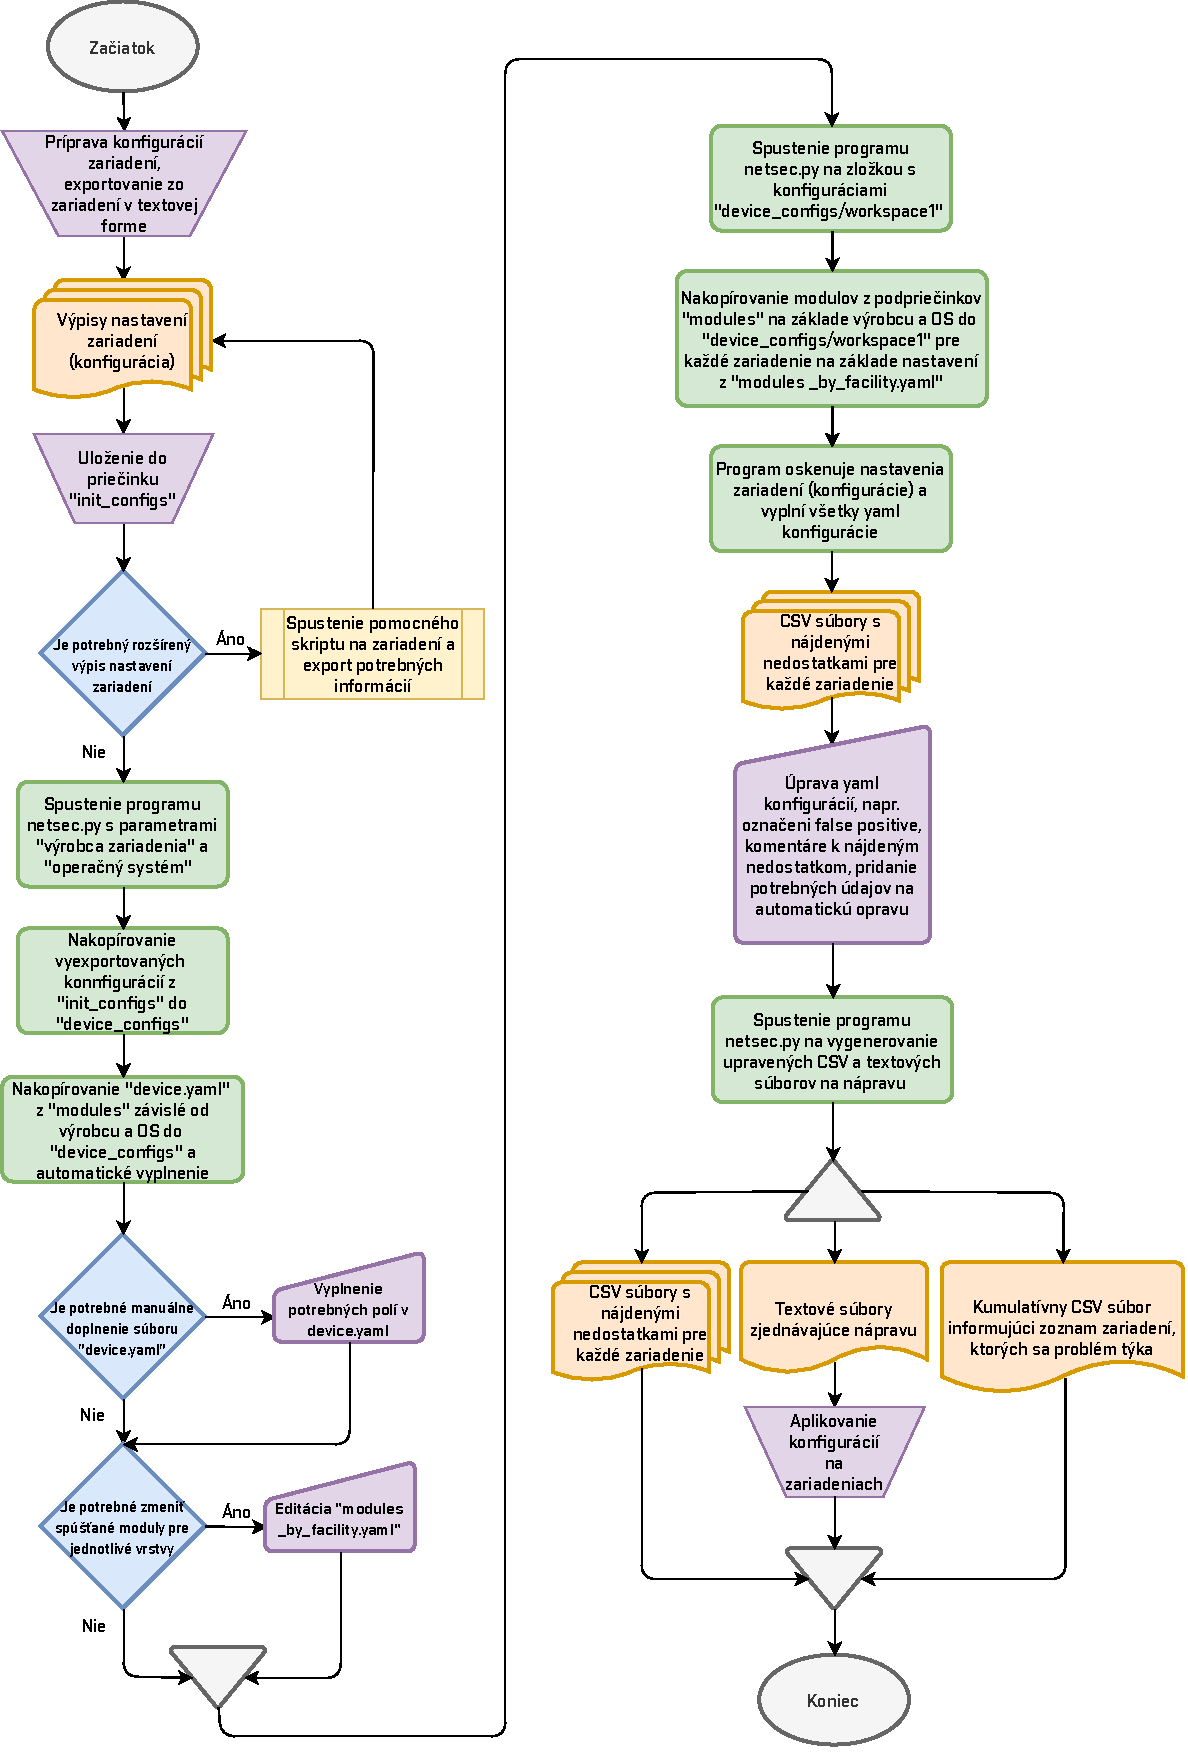
\includegraphics[scale=0.8]{obrazky/flowchart.pdf}
	\end{center}
	\caption[Vývojový diagram opisujúci prácu s~programom a tok dát v~programe]{Vývojový diagram opisujúci prácu s~programom a tok dát v~programe}
	\label{workflow}
\end{figure}

 

\subsection*{Hierarchická štruktúra}
Nasledujúca štruktúra súborov s~komentármi vyobrazuje hierarchiu uloženia potrebných súborov na vykonávanie skenovania nedostatkov a zjednanie náprav. Súbor \texttt{hostname1\_fix\_hash} obsahuje namiesto slova ``hash`` skutočný hash súboru \texttt{hostname1\_config.txt}, aby bolo zrejmé, ku ktorej verzii konfigurácie zariadenia patrí a v~prípade aktualizovania a pridania novej konfigurácie do \texttt{init\_configs} nedošlo k~nejednoznačnosti. Nové konfigurácie stiahnuté zo zariadenia sa schválne nedávajú do zložky \texttt{device\_configs}, keďže táto zložka môže obsahovať už nejakú nápravu a správu k~predchádzajúcej konfigurácie, a preto by mohol vzniknúť konflikt a nebolo by jasné ku ktorej verzii konfigurácie  výstupy programu patria. Program bude uchovávať taktiež históriu jednotlivých skenovaní a náprav, pričom pri iniciovaní nového skenovania a prítomnosti novej verzie konfigurácie zariadenia, príde k~premiestneniu aktuálnych výstupov do podzložky s~hashom prisluchajúcim konfigurácií \texttt{hostname1\_old\_hash}. 
\newpage   
{\small
	%
	\dirtree{%.
		.1 /\DTcomment{koreňový adresár programu}.
		.2 netsec.py\DTcomment{hlavný program}.
		.2 modules\DTcomment{adresár so šablónami konfiguračných súborov}.
		.3 cisco\DTcomment{výrobca sieťového zariadenia}.
		.4 ios\DTcomment{operačný systém bežiaci na zariadení}.
		.5 device.yaml\DTcomment{šalóna na uloženie základných informácií o~zaridení}.
		.5 aaa.
		.6 aaa.py\DTcomment{modul zodpovedný za skenovanie a nápravu}.
		.6 aaa.yaml\DTcomment{šablóna konfiguračného súboru k~modulu}.
		.5 cdp.
		.6 cdp.py.
		.6 cdp.yaml.
		.5 modules\_by\_facility.yaml\DTcomment{súbor s~definíciou, ktoré moduly  budú spustené pre zariadenia na konkrétnej vrstve modelu}.
		.3 hp.
		.3 juniper.
		.4 junos.
		.2 device\_configs\DTcomment{adresár s~výstupmi, konfiguráciami a súbormi na ich nápravu}.
		.3 workspace1\DTcomment{adresár jednej topológie/siete}.
		.4 summary\_report\DTcomment{správa s~mapovaním nedostatok-zariadenie}.
		.4 hostname1.
		.5 device.yaml\DTcomment{základané informácie o~konkrétnom zariadení}.
		.5 aaa.yaml\DTcomment{konfiguračný súbor k~modulu s~nájdenými nedostatkami}.
		.5 cdp.yaml.
		.5 report\_hostname1.csv\DTcomment{detailnejšia správa pre konkrétne zariadenie}.
		.5 version\DTcomment{informácie o~verzii operačného systému a jeho chýb}.
		.5 hostname1\_config.txt\DTcomment{aktuálne skenovaná konfigurácia}.
		.5 hostname1\_fix\_hash\DTcomment{súbor s~nápravnou konfiguráciou}.
		.5 hostname1\_old\_hash\DTcomment{predchádzajúce konfigurácie, zistenie a nápravy}.
		.4 hostname2.
		.3 workspace2.
		.2 init\_configs\DTcomment{adresár s~novými skopírovanými konfiguráciami zariadení}.
		.3 workspace1.
		.4 version.
		.4 hostname1\_config.txt.
		.4 hostname2\_config.txt.
		.3 workspace2.
		.2 current\_output\DTcomment{aktuálne správy a nápravy na jednom mieste}.
		.3 workspace1\_hostname1\_fixhash.
		.3 workspace1\_report\_hostname1.csv.
	}
}

\newpage
\section{Zoznam odporúčaní}

V~súčasnej dobe existuje mnoho odporúčaní, štandardov a benchmarkov, ktoré sa zaoberajú bezpečnosťou a správnou konfiguráciou sieťových zariadení. V~mnohých prípadoch sú buď príliš všeobecné a teda sieťoví inžinieri majú problém zistiť, čo daným odporúčaním autor myslel a ako ho implementovať, alebo sú určené iba pre zariadenia od jedného výrobcu. Problémom je taktiež, že väčšina odporúčaní, štandardov a benchmarkov sa nie úplne prekrývajú, a teda je potrebné pri nastavovaní a audite zariadení čerpať s~mnohých naraz. Nižšie uvedené výsledné tabuľky obsahujú odporúčania z~odbornej literatúry, štandardov a benchmarkov verejne dostupných a používaných v~produkčnom nasadení. Výhodou je aj fakt, že obsahujú odporúčania vychádzajúce z~problémov IPv6, ktoré nie sú často v~štandardoch a benchmarkoch dostupné. Podrobná tabuľka s~mapovaním odporúčaní na príkazy pre zariadenia Cisco s~operačným systémom IOS je v~prílohe TODO príloha %TODO príloha

Zariadenia Cisco boli pre túto prácu vybrané z~dôvodu, že spoločnosť Cisco je lídrom ktorý udáva trend, ich zariadenia sú celosvetovo v~korporáciách veľmi rozšírené a mnoho literatúry a benchmarkov sa odvoláva na nastavenia týchto prístrojov s~udávanými príkladmi konfigurácie. Taktiež sú tieto zariadenia dobrým referenčným príkladom pre hľadanie alternatívy v~zariadeniach od iných výrobcov.

Tabuľky sú rozdelené do skupín podľa protokolu prípadne okruhu problému, ktorému sa venujú. V~tabuľkách je možné vidieť, že odporúčania sú zatriedené podľa viacerých kritérií. V~prvom rade sú to roviny (plane), ktoré nie sú dôležité pre následnú automatickú konfiguráciu a odhaľovanie problémov, ale na vytvorenie si obrazu, ktorá časť rovín je kritická a postihnuteľná najviac. 

Stĺpec závažnosť (severity) vznikol na základe predpokladaných závažností. Tento atribút bude možné zmeniť v~konfiguračnom súbore každého modulu v~závislosti na riziku, ktoré sa pre danú topológiu a firmu vyhodnotí za pomoci manažmentu rizík opísaného v~kapitole \ref{bezpecnostny-audit}. Tento atribút sa nenachádza v~žiadnom štandarde ani benchmarku, z~ktorého vytvorený zoznam odporúčaní čerpal, no je veľmi dôležitý z~hľadiska, že nie všetky nedostatky sú rovnako závažné a nemajú rovnaký dopad. Hodnoty, ktoré nadobúda sú prebrané zo štandardu \zk{zkCVSS}, pričom posledný interval \texttt{none} reprezentujúci nulové riziko respektíve závažnosť je zamenený za kľúčové slovo \texttt{notify}. K~tejto zmene prišlo z~dôvodu, že problémy s~nulovým rizikom nie sú súčasťou návrhu a nemá zmysel ich riešiť. V~prípade, že bude nález falošne pozitívny alebo riziko bude akceptované, tak sa táto skutočnosť uloží do konfiguračného súboru. Závažnosť \texttt{notify} bude použitá v~prípade prítomnosti monitorovania portu pomocou zrkadlenia portu alebo NetFlow/sFlow. Jedná sa totiž o~technológie potrebné na monitorovanie prevádzky z~legislatívnych alebo bezpečnostných dôvodov. Riziko existuje iba pri nesprávnom nastavení zdrojov monitorovania a cieľu pre zber dát, a preto je dobré vedieť pri audite o~prítomnosti tohto nastavenia.
 

Posledným rozdelením je vrstva, na ktorej zariadenie pracuje (facility layer), nakoľko rozdelenie podľa zariadení nie je dostatočné, pretože napríklad L3 prepínač môže byť použitý na ktorejkoľvek vrstve hierarchického modelu a každá vrstva má určité špecifiká, ktoré neobsahuje iná vrstva. Každý konfiguračný súbor popisujúci zariadenie bude obsahovať informáciu, do ktorej vrstvy patrí a na základe toho bude môcť program rozhodnúť, ktoré moduly zodpovedné za nájdenie problému a jeho vyriešenie budú nad konfiguračným súborom zariadenia spustené. Taktiež bude možné meniť, dopĺňať a zakázať spúšťanie modulov pre jednotlivé zariadenia, pokiaľ by v~danej topológii nevyhovovalo rozdelenie z~tabuliek uvedených nižšie. 

Vrstva, na ktorej zariadenie operuje, ako aj definované zariadenie, ktorého sa odporúčanie a opatrenie týka nie sú súčasťou žiadneho kontrolného zoznamu, benchmarku ani štandardu, z~ktorého bolo čerpané. Sieťový administrátor by preto musel sám vyvodiť záver, ktoré odporúčania a postupy bude aplikovať na jednotlivé zariadenia a vrstvy hierarchického modelu. Preto vytvorená tabuľka odporúčaní už obsahuje aj zoznam zariadení, ktorých sa opatrenie týka.

%Z~dôvodu šetrenia priestoru boli hodnoty nadobúdajúce stĺpce Plane a Severity skrátené na iniciály slov reprezentujúce tieto hodnoty. Ich celé názvy je možné nájsť v~kapitole \ref{hierarchydesign} respektíve \ref{riskmanagement}. Stĺpec Facility layer naviac obsahuje hodnotu \texttt{A}, ktorej význam znamená, že toto odporúčanie sa vzťahuje na všetky zariadenia bez ohľadu, na akej vrstve operujú.  

\newpage


\footnotesize
\newgeometry{left=2.7cm,bottom=3.2cm, top=2.5cm}

\begin{longtable}[!htbp]{|C{2.5em}L{11em}L{11em}C{2.5em}C{4em}C{5em}L{2.5em}|}
	\caption{Odporúčania k~prístupu na manažment zariadení}
	\label{tab:managemnet}\\ \hline
	\mbox{Riadok} č.&Útok / Problém	&Mitigácia / Nastavenie	& Plane 	&Severity	&Facility layer	&Zdroj\\ \hhline{=======}
	\endfirsthead 
	\hline
	\centering
	
	Riadok č.	&Útok / Problém	&Mitigácia / Nastavenie	&Plane	&Severity	&Facility layer	&Zdroj\\ \hhline{=======}
	\endhead
	
	\rowcolor[rgb]{ .97,  .97,  .97} 1	&Nepovolený prístup k~manažovaniu zariadenia	&Vytvoriť a aplikovať ACL pre OOB, Telnet, SSH a pod. a zaznamenať v~logu prístupy	&M	&C	&A	& \cite{Akin2002}
	
	\cite{CIS_DrTLsgXv24lxeIIM}	\\
	2	&Neautorizovaný prístup cez nepoužívané a nezabezpečené protokoly na manažment zariadení	&Vypnúť nepoužívané protokoly na prístup k~manažovaniu zariadení (telnet a pod.)	&M	&H	&A	& \cite{CIS_DrTLsgXv24lxeIIM}
	
	\cite{Singh2018}
	\\
	\rowcolor[rgb]{ .97,  .97,  .97} 3	&Nepovolený prístup k~manažmentu konfigurácie zariadenia	&Vypnutie odchádzajúcich spojení pre protokoly na manažment zariadení pokiaľ sa nepoužívajú (telnet a pod.)	&M	&H	&A	& \cite{Singh2018}	\\
	4	&Prístup bez požadovaných prístupových údajov	&Nakonfigurovanie protokolov na manažment zariadení, aby požadovali prístupové údaje (telnet a pod.)	&M	&C	&A	& \cite{CIS_DrTLsgXv24lxeIIM}	\\
	\rowcolor[rgb]{ .97,  .97,  .97} 5	&Nekonzistencia konfiguračných súborov pri zmenách konfigurácie viac ako jedným administrátorom	&Povoliť súčasne iba jednému administrátorovi vykonávanie zmien v~konfigurácii	&M	&H	&A	& \cite{Singh2018}	\\
	6	&Nepoužívanie zabezpečeného protokolu na manažment zariadení môže viesť k~odposluchu	&Zapnutie SSH	&M	&C	&A	& \cite{CIS_DrTLsgXv24lxeIIM}
	
	\cite{Graesser2001}	\\
	\rowcolor[rgb]{ .97,  .97,  .97} 7	&Nebezpečná verzia 1 protokolu SSH	&SSH verzia 2	&M	&C	&A	& \cite{McMillan2018}	\\
	8	&Útok na krátky RSA kľúč	&Dĺžka RSA kľúča minimálne 2048 bitov	&M	&C	&A	& \cite{CIS_DrTLsgXv24lxeIIM}
	
	\cite{Barker2019} 
	\\
	\rowcolor[rgb]{ .97,  .97,  .97} 9	&Dlhé neaktívne sedenie môže byť zneužité alebo aj fyzický prístup útočníka k~aktívnemu sedeniu môže viesť k~zmene konfigurácie	&SSH čas vypršania sedenia	&M	&M	&A	& \cite{CIS_DrTLsgXv24lxeIIM}
	
	\cite{Graesser2001}	\\
	10	&Hádanie hesla k~RSA kľúču	&SSH maximálny počet neúspešných pokusov	&M	&H	&A	& \cite{Hucaby2010}
	
	\cite{Bouska2009}	\\
	\rowcolor[rgb]{ .97,  .97,  .97} 11	&Útok hrubou silou na zistenie prihlasovacích údajov	&Špecifikovať čas po ktorý nie je možné po N pokusoch sa prihlásiť	&M	&H	&A	& \cite{Hucaby2010}
	
	\cite{Bouska2009}	\\
	12	&Prihlásenie na zariadenie nie je možné kvôli zablokovaniu pre príliš veľa neúspešných pokusov	&Povolenie prístupu administrátorovi na základe IP adresy, keď je protokol na manažovanie zariadení nedostupný kvôli DOS útoku	&M	&M	&A	& \cite{Hucaby2010}
	
	\cite{Bouska2009}	\\
	\rowcolor[rgb]{ .97,  .97,  .97} 13	&Dlhé neaktívne sedenie môže byť zneužité alebo aj fyzický prístup útočníka k~aktívnemu sedeniu môže viesť k~zmene konfigurácie	&Čas vypršania sedenia pre protokol na manažovanie zariadení	&M	&M	&A	& \cite{CIS_DrTLsgXv24lxeIIM}
	
	\cite{Graesser2001}
	
	\cite{uYLsMtQInofenpV3}
	\\
	14	&Možné prihlásenie do zariadenia cez telnet keď je prítomné SSH	&Zakázať telnet ak je SSH aktívne	&M	&C	&A	& \cite{CIS_DrTLsgXv24lxeIIM}
	
	\cite{Graesser2001}	\\
	\rowcolor[rgb]{ .97,  .97,  .97} 15	&Útočník nie je informovaný o~právnych následkoch	&Právne upozornenie pri prístupe k~zariadeniu	&M	&L	&A	& \cite{McMillan2018}
	
	\cite{CIS_DrTLsgXv24lxeIIM}
	
	\cite{Graesser2001}	\\
	16	&Nepovolená zmena konfigurácie zariadenia	&Vytvorenie hesla na editovanie konfigurácie zariadenia	&M	&C	&A	& \cite{CIS_DrTLsgXv24lxeIIM}
	
	\cite{Graesser2001}	\\
	\rowcolor[rgb]{ .97,  .97,  .97} 17	&Nepovolený prístup k~manažmentu konfigurácie zariadenia	&Lokálne zabezpečené účty	&M	&C	&A	& \cite{Singh2018}
	
	\cite{CIS_DrTLsgXv24lxeIIM}	\\
	18	&Centrálna správa prihlásení a dohľadateľnosť zmien v~konfigurácií	&Definovanie a povolenie AAA serveru na prihlásenie a definovanie záložného prihlásenia	&M	&H	&A	& \cite{Akin2002}
	
	\cite{CIS_DrTLsgXv24lxeIIM} 
	
	\cite{McMillan2018}
	
	\cite{Graesser2001}	\\
	\rowcolor[rgb]{ .97,  .97,  .97} 19	&Centrálna správa prihlásení a dohľadateľnosť zmien v~konfigurácií	&Definovanie a povolenie AAA serveru na editáciu konfigurácií a definovanie záložného prihlásenia	&M	&M	&A	& \cite{CIS_DrTLsgXv24lxeIIM}
	
	\cite{Graesser2001}	\\
	20	&Hádanie prístupových údajov	&Definovanie maximálneho počtu neúspešných pokusov o~prihlásenie a následné zablokovanie účtu	&M	&H	&A	& \cite{CIS_DrTLsgXv24lxeIIM}
	
	\cite{Graesser2001}	\\
	\rowcolor[rgb]{ .97,  .97,  .97} 21	&Prihlásenie bez prihlasovacích údajov	&Zakázať záložné prihlásenie bez poskytnutia autentifikačných prostriedkov	&M	&C	&A	& \cite{Singh2018}	\\
	22	&AAA používa primárne lokálne účty namiesto centralizovaných na serveri	&AAA nesmie používať ako prvú možnosť prihlásenia lokálny účet 	&M	&H	&A	& \cite{CIS_DrTLsgXv24lxeIIM}
	
	\cite{Graesser2001}	\\
	\rowcolor[rgb]{ .97,  .97,  .97} 23	&Používateľ prihlásený do zariadenia môže spúšťať akékoľvek príkazy	&Nastavenie AAA autorizácie pre spúšťanie príkazov. V~prípade výpadku AAA serveru, bude užívateľ odhlásený a následne prihlásený podľa  záložného prihlásenia, aby mu nebolo pridelené vysoké oprávnenie umožňujúce vykonávať príkazy, na ktoré nemá právo	&M	&H	&A	& \cite{Graesser2001}
	
	\cite{Singh2018}	\\
	24	&Administrátor vloží zlý príkaz a po čase je ho nemožné dohľadať a zjednať nápravu	&Nastavenie AAA účtovania respektíve logovania pripojení a vykonaných príkazov	&M	&H	&A	& \cite{CIS_DrTLsgXv24lxeIIM}	\\
	\rowcolor[rgb]{ .97,  .97,  .97} 25	&AAA zdrojové rozhranie nie je rovnaké pri každom reštarte	&Definovanie loopback zdrojového rozhrania pre AAA	&M	&M	&A	& \cite{CIS_DrTLsgXv24lxeIIM}	\\
	26	&SSH zdrojové rozhranie nie je rovnaké pri každom reštarte	& Definovanie loopback zdrojového rozhrania pre SSH	&M	&M	&A	& \cite{CIS_DrTLsgXv24lxeIIM}	\\
	\rowcolor[rgb]{ .97,  .97,  .97} 27	&DOS útok na štandardný SSH port 22	&Špecifikovanie iného portu pre SSH ako štandardného alebo aplikovanie Port Knocking \cite{MJVmQiKUgZl92S8u}	&M	&H	&A	& \cite{MJVmQiKUgZl92S8u}	\\
	\hline
	
	
\end{longtable}%
\vspace{-1em}
{\tiny 
	\noindent
	Plane: M\,--\,Management, C\,--\,Control, D\,--\,Data\\
	Severity: C\,--\,Critical, H\,--\,High, M\,--\,Medium, L\,--\,Low, N\,--\,Notify\\
	Facility layer: A\,--\,Všetky zariadenia, CE\,--\,Core/Edge, DI\,--\,Distribution, AC\,--\,Access, CAL\,--\,Collapsed All, CDA\,--\,Collapsed Distribution Access, CCD\,--\,Collapsed Core Distribution}


\begin{longtable}[!htbp]{|C{2.5em}L{11em}L{11em}C{2.5em}C{4em}C{5em}L{2.5em}|}
	\caption{Odporúčania pre smerovanie}
	\label{tab:routing}\\ \hline
	\mbox{Riadok} č.&Útok / Problém	&Mitigácia / Nastavenie	&Plane	&Severity	&Facility layer	&Zdroj\\ \hhline{=======}
	\endfirsthead 
	\hline
	\centering
	
	Riadok č.	&Útok / Problém	&Mitigácia / Nastavenie	&Plane	&Severity	&Facility layer	&Zdroj\\ \hhline{=======}
	\endhead
	
	\rowcolor[rgb]{ .97,  .97,  .97} 1	&Vloženie a manipulácia so smerovacími informáciami	&Autentifikácia smerovacích protokolov (nie heslá v~otvorenej podobe)	&C	&H	&CE,
	DI,
	CCD,
	CDA,
	CAL	& \cite{McMillan2018}
	
	\cite{Singh2018}
	
	\cite{CIS_DrTLsgXv24lxeIIM}\\
	2	&OSPF virtuálne linky degradujú výkon	&Vypnutie virtuálnych liniek pre OSPF	&C	&H	&CE,
	DI,
	CCD,
	CDA,
	CAL	& \cite{Tiso2012}\\
	\rowcolor[rgb]{ .97,  .97,  .97} 3	&Koncové zariadenie, užívateľ a útočník môžu vidieť smerovacie správy a topológiu siete alebo pripojenie škodlivého zariadenia, ktoré vysielať a prijímať smerovacie správy	&Špecifikovanie rozhraní, ktoré nebudú prijímať smerovacie informácie	&C	&H	&CE,
	DI,
	CCD,
	CDA,
	CAL	& \cite{Khandelwal2016}\\
	4	&Nemožnosť sprevádzkovať procesy smerovacích protokolov v~určitých prípadoch pri použití IPv6	&Špecifikovanie identifikátorov smerovacích protokolov pre každý router (router ID)	&C	&M	&CE,
	DI,
	CCD,
	CDA,
	CAL	& \cite{q7WZuvqA1fZEsYyL}
	
	\cite{Lammle2013}\\
	\rowcolor[rgb]{ .97,  .97,  .97} 5	&Vysledovateľnosť nefunkčnosti smerovacieho protokolu a nesprávneho nastavenia	&Zaznamenanie zmeny v~logu pri zmenách v~smerovaní	&C	&M	&CE,
	DI,
	CCD,
	CDA,
	CAL	& \cite{uYLsMtQInofenpV3}
	\\
	6	& Škodlivé vloženie smerovacích informácií informácií, vzdialený útok	&TTL security	&C	&H	&CE,
	DI,
	CCD,
	CDA,
	CAL	& \cite{Khandelwal2016}
	
	\cite{Singh2018}\\
	\rowcolor[rgb]{ .97,  .97,  .97} 7	&Nesprávne smerovanie kvôli sumarizácií	&Vypnutie automatickej sumarizácie smerovacích protokolov	&C	&H	&CE,
	DI,
	CCD,
	CDA,
	CAL	& \cite{Lammle2013}\\
	8	&DOS útok na stanicu, cez ktorú bola špecifikovaná cesta a teda nemožnosť komunikácie s~koncovým bodom. Alebo zosnovanie MITM útoku	&Vypnutie IP source routing	&C	&C	&CE,
	DI,
	CCD,
	CDA,
	CAL	& \cite{CIS_DrTLsgXv24lxeIIM}\\
	\rowcolor[rgb]{ .97,  .97,  .97} 9	&DOS útok pomocou podvrhnutej IP adresy alebo vzdialený útok na smerovací protokol	&Zapnutie reverse path forwarding strict/loose mode	&C	&H	&CE,
	DI,
	CCD,
	CDA,
	CAL	& \cite{Khandelwal2016}
	
	\cite{Jackson2010}
	
	\cite{CIS_DrTLsgXv24lxeIIM}\\
	
	\hline
	
\end{longtable}%
\vspace{-1em}
{\tiny 
	\noindent
	Plane: M\,--\,Management, C\,--\,Control, D\,--\,Data\\
	Severity: C\,--\,Critical, H\,--\,High, M\,--\,Medium, L\,--\,Low, N\,--\,Notify\\
	Facility layer: A\,--\,Všetky zariadenia, CE\,--\,Core/Edge, DI\,--\,Distribution, AC\,--\,Access, CAL\,--\,Collapsed All, CDA\,--\,Collapsed Distribution Access, CCD\,--\,Collapsed Core Distribution}

\begin{longtable}[!htbp]{|C{2.5em}L{11em}L{11em}C{2.5em}C{4em}C{5em}L{2.5em}|}
	\caption{Odporúčania pre filtrovanie prevádzky}
	\label{tab:filtering}\\ \hline
	\mbox{Riadok} č.&Útok / Problém	&Mitigácia / Nastavenie	&Plane	&Severity	&Facility layer	&Zdroj\\ \hhline{=======}
	\endfirsthead 
	\hline
	\centering
	
	Riadok č.	&Útok / Problém	&Mitigácia / Nastavenie	&Plane	&Severity	&Facility layer	&Zdroj\\ \hhline{=======}
	\endhead
	
	
	\rowcolor[rgb]{ .97,  .97,  .97} 1	&IP spoofing	&Špecifikácia ACL na zakázanie a logovanie privátnych a špeciálnych IP adries z~RFC 1918, RFC 3330	&C	&C	&CE,
	CCD,
	CAL	& \cite{Jackson2010}
	
	\cite{Singh2018}
	
	\cite{CIS_DrTLsgXv24lxeIIM}\\
	2	&IP spoofing	&Špecifikácia ACL na zakázanie a logovanie špeciálnych IPv6 adries z~RFC 5156	&C	&C	&CE,
	CCD,
	CAL	& \cite{Jackson2010}
	
	\cite{Singh2018}
	
	\cite{CIS_DrTLsgXv24lxeIIM}\\
	\rowcolor[rgb]{ .97,  .97,  .97} 3	&IPv6 Next Header,
	IPv6 Fragmentation útok	&ACL blokujúce nerozpoznateľné rozšírené hlavičky	&C	&C	&A	& \cite{Podermanski1922015}
	
	\cite{Gregr2622015}\\
	4	&DOS útok alebo pokus o~prístup k~tomu, čo nie je povolené	&Logovanie pravidiel zahodenia paketov v~ACL	&M	&M	&A	& \cite{Akin2002}\\
	\rowcolor[rgb]{ .97,  .97,  .97} 5	&Pakety budú spracovávané v~CPU, ktoré môže byť preťažené a môže byť zmenené smerovanie na obídenie bezpečnostnej kontroly	&Zahadzovanie IPv4 paketov s~rozšírenou hlavičkou (IP Options filtering)	&C	&C	&CE,
	DI,
	CCD,
	CDA,
	CAL	& \cite{Singh2018}\\
	6	&Komplexné bezpečnostné hrozby a narušenie bezpečnosti	&Nastavenie IDS/IPS ak to zariadenie podporuje	&C	&H	&CE, CCD,
	CAL	& \cite{Hucaby2010}\\
	\hline
\end{longtable}%
\vspace{-1em}
{\tiny 
	\noindent
	Plane: M\,--\,Management, C\,--\,Control, D\,--\,Data\\
	Severity: C\,--\,Critical, H\,--\,High, M\,--\,Medium, L\,--\,Low, N\,--\,Notify\\
	Facility layer: A\,--\,Všetky zariadenia, CE\,--\,Core/Edge, DI\,--\,Distribution, AC\,--\,Access, CAL\,--\,Collapsed All, CDA\,--\,Collapsed Distribution Access, CCD\,--\,Collapsed Core Distribution}

\begin{longtable}[!htbp]{|C{2.5em}L{11em}L{11em}C{2.5em}C{4em}C{5em}L{2.5em}|}
	\caption{Odporúčania pri vysokom zaťažení}
	\label{tab:highload}\\ \hline
	\mbox{Riadok} č.&Útok / Problém	&Mitigácia / Nastavenie	&Plane	&Severity	&Facility layer	&Zdroj\\ \hhline{=======}
	\endfirsthead 
	\hline
	\centering
	
	Riadok č.	&Útok / Problém	&Mitigácia / Nastavenie	&Plane	&Severity	&Facility layer	&Zdroj\\ \hhline{=======}
	\endhead
	
	\rowcolor[rgb]{ .97,  .97,  .97} 1	&Nízky stav voľnej pamäte	&Nastavenie notifikácie pri dochádzaní pamäte	&M	&M	&A	& \cite{Singh2018}
	
	\cite{uYLsMtQInofenpV3}\\
	2	&Logovacie správy nemôžu byť zaznamenané kvôli nedostatku pamäte	&Rezervovanie pamäte pre kritické notifikácie pri nedostatku pamäte	&M	&H	&A	& \cite{Singh2018}
	
	\cite{uYLsMtQInofenpV3}\\
	\rowcolor[rgb]{ .97,  .97,  .97} 3	&Vysoké zaťaženie CPU	&Nastavenie notifikácie vysokom zaťažení CPU	&M	&M	&A	& \cite{Singh2018}
	
	\cite{uYLsMtQInofenpV3}\\
	4	&Vysoké zaťaženie zariadenia spôsobilo nemožnosť prihlásenia k~nemu	&Rezervovanie pamäte pre protokoly na manažment zariadení pri nedostatku pamäte	&M	&H	&A	& \cite{Singh2018}\\	
	\hline
\end{longtable}%
\vspace{-1em}
{\tiny 
	\noindent
	Plane: M\,--\,Management, C\,--\,Control, D\,--\,Data\\
	Severity: C\,--\,Critical, H\,--\,High, M\,--\,Medium, L\,--\,Low, N\,--\,Notify\\
	Facility layer: A\,--\,Všetky zariadenia, CE\,--\,Core/Edge, DI\,--\,Distribution, AC\,--\,Access, CAL\,--\,Collapsed All, CDA\,--\,Collapsed Distribution Access, CCD\,--\,Collapsed Core Distribution}

\begin{longtable}[!htbp]{|C{2.5em}L{11em}L{11em}C{2.5em}C{4em}C{5em}L{2.5em}|}
	\caption{Odporúčania na zamedzenie mapovanie siete}
	\label{tab:mapping}\\ \hline
	\mbox{Riadok} č.&Útok / Problém	&Mitigácia / Nastavenie	&Plane	&Severity	&Facility layer	&Zdroj\\ \hhline{=======}
	\endfirsthead 
	\hline
	\centering
	
	Riadok č.	&Útok / Problém	&Mitigácia / Nastavenie	&Plane	&Severity	&Facility layer	&Zdroj\\ \hhline{=======}
	\endhead
	
	\rowcolor[rgb]{ .97,  .97,  .97} 1	&Skenovanie a zistenie informácií o~sieti za pomoci protokolu CDP a využitie bezpečnostných chýb	&Zakázanie protokolu CDP	&M	&C	&A	& \cite{CIS_DrTLsgXv24lxeIIM}
	
	\cite{Graesser2001}\\
	2	&Skenovanie a zistenie informácií o~sieti za pomoci protokolu LLDP a využitie bezpečnostných chýb	&Zakázanie protokolu LLDP	&M	&C	&A	& \cite{McMillan2018}\\
	\rowcolor[rgb]{ .97,  .97,  .97} 3	&Proxy ARP môže viesť k~obídeniu PVLAN a rozširuje broadcast doménu	&Vypnutie Proxy ARP	&C	&C	&CE,
	DI,
	CCD,
	CDA,
	CAL	& \cite{CIS_DrTLsgXv24lxeIIM}
	
	\cite{Graesser2001}\\
	4	&Útočník môže zistiť, že IP adresa, na ktorú skúšal ping je nesprávna	&Vypnutie správ ICMP Unreachable	&D	&H	&CE,
	DI,
	CCD,
	CDA,
	CAL	& \cite{Singh2018}
	\\
	\rowcolor[rgb]{ .97,  .97,  .97} 5	&Útočník môže zistiť masku podsiete pomocou ICMP Mask reply	&Vypnutie správ ICMP Mask reply	&D	&H	&CE,
	DI,
	CCD,
	CDA,
	CAL	& \cite{Akin2002}
	\\
	6	&Umožňuje DOS Smurf útok, mapovanie siete pomocou ping na broadcast adresu vzdialenej siete	&Vypnutie ICMP echo správ na broadcast adresu, vypnutie directed broadcasts	&D	&C	&CE,
	DI,
	CCD,
	CDA,
	CAL	& \cite{Graesser2001}
	
	\cite{Akin2002}
	\\
	\rowcolor[rgb]{ .97,  .97,  .97} 7	&Útočník môže zistiť smerovacie informácie alebo vyťažiť CPU	&Vypnutie správ ICMP Redirects	&D	&H	&CE,
	DI,
	CCD,
	CDA,
	CAL	& \cite{Singh2018}
	\\
	8	&Mapovanie siete pomocou pingu na multicast adresu všetkých uzlov a MLD/IGMP Query Overload a Smurf útok	& ACL blokujúce ICMP echo request na multicast adresu všetkých uzlov a MLD/IGMP Query na prístupových portoch	&C	&M	&DI,
	CDA,
	AC	&\cite{Podermanski532015}
	
	\cite{Rey2016}\\
	\hline
\end{longtable}%
\vspace{-1em}
{\tiny 
	\noindent
	Plane: M\,--\,Management, C\,--\,Control, D\,--\,Data\\
	Severity: C\,--\,Critical, H\,--\,High, M\,--\,Medium, L\,--\,Low, N\,--\,Notify\\
	Facility layer: A\,--\,Všetky zariadenia, CE\,--\,Core/Edge, DI\,--\,Distribution, AC\,--\,Access, CAL\,--\,Collapsed All, CDA\,--\,Collapsed Distribution Access, CCD\,--\,Collapsed Core Distribution}

\begin{longtable}[!htbp]{|C{2.5em}L{11em}L{11em}C{2.5em}C{4em}C{5em}L{2.5em}|}
	\caption{Odporúčania na identifikáciu zariadení a nastavení}
	\label{tab:identification}\\ \hline
	\mbox{Riadok} č.&Útok / Problém	&Mitigácia / Nastavenie	&Plane	&Severity	&Facility layer	&Zdroj\\ \hhline{=======}
	\endfirsthead 
	\hline
	\centering
	
	Riadok č.	&Útok / Problém	&Mitigácia / Nastavenie	&Plane	&Severity	&Facility layer	&Zdroj\\ \hhline{=======}
	\endhead
	
	\rowcolor[rgb]{ .97,  .97,  .97} 1	&Nemožná identifikácia zariadenia	&Vytvoriť hostname	&M	&L	&A	& \cite{CIS_DrTLsgXv24lxeIIM}\\
	2	&Nemožnosť vzdialeného prístupu	&Vytvoriť doménové meno	&M	&L	&A	& \cite{CIS_DrTLsgXv24lxeIIM}\\
	\rowcolor[rgb]{ .97,  .97,  .97} 3	&Identifikácia pravidla v~ACL	&Popis každého pravidla v~ACL pre lepšiu identifikáciu	&M	&L	&A	& \cite{Singh2018}\\
	4	&Identifikácia rozhrania	&Popis každého rozhrania	&M	&L	&A	& \cite{Lammle2013}\\
	\rowcolor[rgb]{ .97,  .97,  .97} 5	&Nemožnosť identifikácie účelu VLAN	&Pridanie mena k~VLAN	&C	&L	&DI,
	CDA,
	AC,
	
	CAL	& \cite{Lammle2013}\\	
	\hline
\end{longtable}%
\vspace{-1em}
{\tiny 
	\noindent
	Plane: M\,--\,Management, C\,--\,Control, D\,--\,Data\\
	Severity: C\,--\,Critical, H\,--\,High, M\,--\,Medium, L\,--\,Low, N\,--\,Notify\\
	Facility layer: A\,--\,Všetky zariadenia, CE\,--\,Core/Edge, DI\,--\,Distribution, AC\,--\,Access, CAL\,--\,Collapsed All, CDA\,--\,Collapsed Distribution Access, CCD\,--\,Collapsed Core Distribution}


\begin{longtable}[!htbp]{|C{2.5em}L{11em}L{11em}C{2.5em}C{4em}C{5em}L{2.5em}|}
	
	\caption{Odporúčania k~protokolu NTP}
	\label{tab:ntp}\\ \hline
	\mbox{Riadok} č.&Útok / Problém	&Mitigácia / Nastavenie	&Plane	&Severity	&Facility layer	&Zdroj\\ \hhline{=======}
	\endfirsthead 
	\hline
	\centering
	
	Riadok č.	&Útok / Problém	&Mitigácia / Nastavenie	&Plane	&Severity	&Facility layer	&Zdroj\\ \hhline{=======}
	\endhead
	
	\rowcolor[rgb]{ .97,  .97,  .97} 1	&Nekonzistencia časov v~logoch a problém pričlenenia logov k~relevantným incidentom	&Nastavenie NTP serveru pre aktuálny čas v~logoch	&M	&H	&A	& \cite{Jackson2010}
	
	\cite{Singh2018}
	
	\cite{CIS_DrTLsgXv24lxeIIM}\\
	2	&Pripojenie servera s~rovnakou IP adresou, ale falošným časom	&Nastavenie NTP autentifikácie	&M	&H	&A	& \cite{Jackson2010}
	
	\cite{Singh2018}
	
	\cite{CIS_DrTLsgXv24lxeIIM}\\
	\rowcolor[rgb]{ .97,  .97,  .97} 3	&NTP zdrojové rozhranie nie je rovnaké pri každom reštarte	& Definovanie loopback zdrojového rozhrania pre NTP	&M	&M	&A	& \cite{Jackson2010}
	
	\cite{Singh2018}
	
	\cite{CIS_DrTLsgXv24lxeIIM}\\
	4	&Väčšia bezpečnosť (pub/priv key) NTP a podpora IPv6	&Použitie NTP verzie 4	&M	&M	&A	&\cite{s0goWNnWp5OjqREE}\\
	\rowcolor[rgb]{ .97,  .97,  .97} 5	&Falošný čas od podvrhnutého NTP zdroja	&Nastavenie NTP peer s~inými sieťovými zariadeniami na krížovú validáciu času a záložný zdroj času	&M	&M	&A	& \cite{Akin2002}\\
	\hline
\end{longtable}%
\vspace{-1em}
{\tiny 
	\noindent
	Plane: M\,--\,Management, C\,--\,Control, D\,--\,Data\\
	Severity: C\,--\,Critical, H\,--\,High, M\,--\,Medium, L\,--\,Low, N\,--\,Notify\\
	Facility layer: A\,--\,Všetky zariadenia, CE\,--\,Core/Edge, DI\,--\,Distribution, AC\,--\,Access, CAL\,--\,Collapsed All, CDA\,--\,Collapsed Distribution Access, CCD\,--\,Collapsed Core Distribution}

\begin{longtable}[!htbp]{|C{2.5em}L{11em}L{11em}C{2.5em}C{4em}C{5em}L{2.5em}|}
	
	\caption{Odporúčanie pre protokol SNMP}
	\label{tab:snmp}\\ \hline
	\mbox{Riadok} č.&Útok / Problém	&Mitigácia / Nastavenie	&Plane	&Severity	&Facility layer	&Zdroj\\ \hhline{=======}
	\endfirsthead 
	\hline
	\centering
	
	Riadok č.	&Útok / Problém	&Mitigácia / Nastavenie	&Plane	&Severity	&Facility layer	&Zdroj\\ \hhline{=======}
	\endhead
	
	\rowcolor[rgb]{ .97,  .97,  .97} 1	&Odpočúvanie SNMP verzie 1 a 2c	&Použitie SNMP verzie 3 pokiaľ je SNMP používané	&M	&C	&A	& \cite{CIS_DrTLsgXv24lxeIIM}
	
	\cite{Graesser2001}\\
	2	&Modifikovanie konfigurácie pomocou SNMP	&Obmedzenie SNMP iba na čítanie	&M	&C	&A	& \cite{CIS_DrTLsgXv24lxeIIM}
	
	\cite{Graesser2001}
	
	\cite{Akin2002}\\
	\rowcolor[rgb]{ .97,  .97,  .97} 3	&Neoprávnený prístup k~SNMP informáciám	&Obmedzenie SNMP iba pre vybrané IP adresy	&M	&H	&A	& \cite{CIS_DrTLsgXv24lxeIIM}
	
	\cite{Graesser2001}\\
	4	&Administrátor nemá povedomie o~problémoch na zariadení	&Povolenie asynchrónnych správ SNMP TRAP	&M	&M	&A	& \cite{CIS_DrTLsgXv24lxeIIM}
	
	\cite{Graesser2001}
	
	\cite{Akin2002}\\
	\rowcolor[rgb]{ .97,  .97,  .97} 5	&Odpočúvanie SNMP sedenie z~dôvodu slabého šifrovania a hashovacej  funkcie	&Vytvorenie SNMP verzie 3 užívateľa s~minimálnym šifrovaním AES 128 bit a hashovacou funkciou SHA	&M	&C	&A	& \cite{Barker2019}
	
	\cite{CIS_DrTLsgXv24lxeIIM}
	
	\cite{Akin2002}\\
	6	&Sťažená identifikácia SNMP správ z~rôznych IP	&Definovanie lokácie SNMP serveru	&M	&L	&A	& \cite{Dooley2007}\\
	\rowcolor[rgb]{ .97,  .97,  .97} 7	&SNMP zdrojové rozhranie nie je rovnaké pri každom reštarte	& Definovanie loopback zdrojového rozhrania pre SNMP	&M	&M	&A	& \cite{CIS_DrTLsgXv24lxeIIM}\\
	8	&Zmeny názvov rozhraní medzi reštartami a nemožnosť monitorovania pomocou SNMP	&SNMP statické nemenné meno rozhrania aj po reštarte zariadenia	&M	&H	&A	& \cite{Dooley2007}\\
	
	\hline
\end{longtable}%
\vspace{-1em}
{\tiny 
	\noindent
	Plane: M\,--\,Management, C\,--\,Control, D\,--\,Data\\
	Severity: C\,--\,Critical, H\,--\,High, M\,--\,Medium, L\,--\,Low, N\,--\,Notify\\
	Facility layer: A\,--\,Všetky zariadenia, CE\,--\,Core/Edge, DI\,--\,Distribution, AC\,--\,Access, CAL\,--\,Collapsed All, CDA\,--\,Collapsed Distribution Access, CCD\,--\,Collapsed Core Distribution}

\begin{longtable}[!htbp]{|C{2.5em}L{11em}L{11em}C{2.5em}C{4em}C{5em}L{2.5em}|}
	
	\caption{Odporúčania pre protokol Syslog}
	\label{tab:syslog}\\ \hline
	\mbox{Riadok} č.&Útok / Problém	&Mitigácia / Nastavenie	&Plane	&Severity	&Facility layer	&Zdroj\\ \hhline{=======}
	\endfirsthead 
	\hline
	\centering
	
	Riadok č.	&Útok / Problém	&Mitigácia / Nastavenie	&Plane	&Severity	&Facility layer	&Zdroj\\ \hhline{=======}
	\endhead
	
	\rowcolor[rgb]{ .97,  .97,  .97} 1	&Administrátor nemá povedomie o~problémoch na zariadení	&Povolenie logovania protokolom SYSLOG a špecifikovanie IP adresy SYSLOG serveru	&M	&H	&A	& \cite{CIS_DrTLsgXv24lxeIIM}
	
	\cite{Graesser2001}\\
	2	&Neprijímanie všetkých dôležitých incidentov na zariadení z~protokolu SYSLOG	&Špecifikovanie dôležitosti oznámení SYSLOG na INFORMATIONAL	&M	&M	&A	& \cite{CIS_DrTLsgXv24lxeIIM}\\
	\rowcolor[rgb]{ .97,  .97,  .97} 3	&SYSLOG zdrojové rozhranie nie je rovnaké pri každom reštarte	& Definovanie loopback zdrojového rozhrania pre SYSLOG	&M	&M	&A	& \cite{Singh2018}
	
	\cite{CIS_DrTLsgXv24lxeIIM}\\
	4	&Insufficient and non-standard  time format in logging messages/ Nedostatočné a neštandardné formáty času pri logovacích správach	&Definovanie formátu času pre logovacie a ladiace výstupy	&M	&M	&A	& \cite{CIS_DrTLsgXv24lxeIIM}
	
	\cite{Graesser2001}\\
	\rowcolor[rgb]{ .97,  .97,  .97} 5	&Administrátor nevidí dôležité incidenty pri prihlásení a konfigurovaní cez konzolu	&Vypisovanie SYSLOG správ CRITICAL a dôležitejších do terminálu	&M	&M	&A	& \cite{Singh2018}
	
	\cite{CIS_DrTLsgXv24lxeIIM}\\
	6	&Malá vyrovnávacia pamäť pre SYSLOG je dôvodom zahadzovanie správ	&Definovanie veľkosti SYSLOG buffera dôležitosti oznámení na INFORMATIONAL	&M	&H	&A	& \cite{Singh2018}\\
	\rowcolor[rgb]{ .97,  .97,  .97} 7	&Neprístupný SYSLOG server spôsobuje zahadzovanie dôležitých syslog správ	&Definovanie dočasného úložiska SYSLOG správ v~prípade nedostupnosti servera	&M	&H	&A	& \cite{Singh2018}\\
	8	&Problém identifikácie SYSLOG správ s~rovnakou časovou značkou	&Pridanie sekvenčného čísla ku každej syslog správe	&M	&L	&A	& \cite{Akin2002}\\
	
	\hline
\end{longtable}%
\vspace{-1em}
{\tiny 
	\noindent
	Plane: M\,--\,Management, C\,--\,Control, D\,--\,Data\\
	Severity: C\,--\,Critical, H\,--\,High, M\,--\,Medium, L\,--\,Low, N\,--\,Notify\\
	Facility layer: A\,--\,Všetky zariadenia, CE\,--\,Core/Edge, DI\,--\,Distribution, AC\,--\,Access, CAL\,--\,Collapsed All, CDA\,--\,Collapsed Distribution Access, CCD\,--\,Collapsed Core Distribution}

\
\begin{longtable}[!htbp]{|C{2.5em}L{11em}L{11em}C{2.5em}C{4em}C{5em}L{2.5em}|}
	
	\caption{First Hop Security útoky a odporúčania}
	\label{tab:fhs}\\ \hline
	\mbox{Riadok} č.&Útok / Problém	&Mitigácia / Nastavenie	&Plane	&Severity	&Facility layer	&Zdroj\\ \hhline{=======}
	\endfirsthead 
	\hline
	\centering
	
	Riadok č.	&Útok / Problém	&Mitigácia / Nastavenie	&Plane	&Severity	&Facility layer	&Zdroj\\ \hhline{=======}
	\endhead
	
	\rowcolor[rgb]{ .97,  .97,  .97} 1	&MAC Spoofing, MAC Flooding 	&Definovanie maximálne 1 MAC adresy na port, priradenie MAC adresy na port	&C	&C	&DI,
	CDA,
	AC	& \cite{Lammle2013}\\
	2	&MAC Spoofing, MAC Flooding 	&Nastavenie režimu narušenia, ktorý vypne port alebo informuje správcu o~pripojení nepovoleného zariadenia	&C	&H	&DI,
	CDA,
	AC	& \cite{Lammle2013}\\
	\rowcolor[rgb]{ .97,  .97,  .97} 3	&Využívanie siete nepovolenými používateľmi	&Zapnutie 802.1x 	&C	&H	&DI,
	CDA,
	AC	& \cite{Vyncke2008}
	
	\cite{Bouska20071}
	
	\cite{Bouska2007} \\
	4	&Útok hrubou silou hádaním prístupových údajov pre 802.1x 	&Limitovanie maximálneho počtu neúspešných pokusov o~autentifikáciu 802.1x	&C	&H	&DI,
	CDA,
	AC	& \cite{Vyncke2008}
	
	\cite{Bouska20071}
	
	\cite{Bouska2007} \\
	\rowcolor[rgb]{ .97,  .97,  .97} 5	&DHCP spoofing	&DHCP snooping, IPv6 Snooping, DHCPv6 Guard	&C	&C	&DI,
	CDA,
	AC	& \cite{Vyncke2008}
	
	\cite{Singh2018} 
	
	\cite{zXCpMaLbN1J7D1z2}\\
	6	&Príliš veľa DHCP paketov, zaplavenie DHCP paketmi	&Obmedziť počet DHCP paketov na nedôveryhodných rozhraniach	&C	&M	&DI,
	CDA,
	AC	& \cite{Vyncke2008}
	
	\cite{Singh2018}
	
	\cite{zXCpMaLbN1J7D1z2}\\
	\rowcolor[rgb]{ .97,  .97,  .97} 7	&ARP Spoofing	&Dynamic ARP Inspection	&C	&C	&DI,
	CDA,
	AC	& \cite{McMillan2018}\\
	8	&IP spoofing	&IPv4/IPv6 Source Guard	&C	&C	&DI,
	CDA,
	AC	& \cite{Singh2018}
	
	\cite{zXCpMaLbN1J7D1z2}\\
	\rowcolor[rgb]{ .97,  .97,  .97} 9	&IPv6 ND Spoofing	&IPv6 ND Inspection	&C	&C	&DI,
	CDA,
	AC	&\cite{Podermanski1222015}
	
	\cite{Gregr522015}
	
	\cite{zXCpMaLbN1J7D1z2}\\
	10	&Rogue RA,
	
	RA Flood,
	
	RouterLifeTime=0
	&RA Guard	&C	&C	&DI,
	CDA,
	AC	&\cite{Podermanski1222015}
	
	\cite{Gregr522015}
	
	\cite{zXCpMaLbN1J7D1z2}\\
	\rowcolor[rgb]{ .97,  .97,  .97} 11	&Mobilné zariadenia pripojené bezdrôtovo spotrebovávajú veľa energie kvôli častým RA správam	&RA Throttling	&C	&L	&DI,
	CDA,
	AC	& \cite{Podermanski532015}
	
	\cite{o31nYG4kn98wWNRS}\\
	12	&Vyčerpanie cache susedov	&Statický záznam pre kritické zariadenia (servery) spájajúce IP a MAC adresu a VLAN
	&C	&C	&DI,
	CDA,
	AC	&\cite{Podermanski1232015}
	
	\cite{Podermanski1932015}
	\\
	\rowcolor[rgb]{ .97,  .97,  .97} 13	&Vyčerpanie cache susedov	&Na zabránenie vzdialeného útoku na cache susedov cez internet je potreba nastaviť ACL, kde povoľujeme iba komunikáciu s~cieľovými IPv6 adresami, ktoré sa nachádzajú v~našej sieti	&C	&C	&CE,
	CCD,
	CAL	&\cite{Podermanski1232015}
	
	\cite{Podermanski1932015}
	\\
	14	&Vyčerpanie cache susedov	&IP destination Guard (First Hop Security)
	
	
	&C	&C	&DI,
	CDA,
	AC	&\cite{Podermanski1232015}
	
	\cite{Podermanski1932015}
	\\
	\rowcolor[rgb]{ .97,  .97,  .97} 15	&Vyčerpanie cache susedov	&Limitovanie času IPv6 adresy v~cache susedov	&C	&C	&DI,
	CDA,
	AC	&\cite{Podermanski1232015}
	
	\cite{Podermanski1932015}\\ 
	\hline
\end{longtable}%
\vspace{-1em}
{\tiny 
	\noindent
	Plane: M\,--\,Management, C\,--\,Control, D\,--\,Data\\
	Severity: C\,--\,Critical, H\,--\,High, M\,--\,Medium, L\,--\,Low, N\,--\,Notify\\
	Facility layer: A\,--\,Všetky zariadenia, CE\,--\,Core/Edge, DI\,--\,Distribution, AC\,--\,Access, CAL\,--\,Collapsed All, CDA\,--\,Collapsed Distribution Access, CCD\,--\,Collapsed Core Distribution}


\begin{longtable}[!htbp]{|C{2.5em}L{11em}L{11em}C{2.5em}C{4em}C{5em}L{2.5em}|}
	
	\caption{Odporúčania pre Spanning Tree Protokol}
	\label{tab:stp}\\ \hline
	\mbox{Riadok} č.&Útok / Problém	&Mitigácia / Nastavenie	&Plane	&Severity	&Facility layer	&Zdroj\\ \hhline{=======}
	\endfirsthead 
	\hline
	\centering
	
	Riadok č.	&Útok / Problém	&Mitigácia / Nastavenie	&Plane	&Severity	&Facility layer	&Zdroj\\ \hhline{=======}
	\endhead
	
	Riadok č.	&Útok / Problém	&Mitigácia / Nastavenie	&Plane	&Severity	&Facility layer	&Zdroj\\
	\endhead
	
	\rowcolor[rgb]{ .97,  .97,  .97} 1	&Rogue root bridge protection (root guard)	&Rogue root bridge 	&C	&C	&DI,
	CDA,
	AC	& \cite{Vyncke2008}\\
	2	&BPDU protection (BPDU guard)	&Pripojenie prepínaču na koncový prístupový port	&C	&C	&DI,
	CDA,
	AC	& \cite{Vyncke2008}\\
	\rowcolor[rgb]{ .97,  .97,  .97} 3	&Prístupové porty by sa nemali podieľať na STP procese	&Rýchlosť konvergencie	&C	&H	&DI,
	CDA,
	AC	& \cite{Vyncke2008}\\
	4	&Špeciálne konfigurácie zaisťujúce bezslučkovú topológiu pomocou STP keď nastane jednosmerná komunikácia (Loop Guard)	&Jednosmerná komunikácia medzi prepínačmi môže viesť k~topológii so slučkami	&C	&C	&DI,
	CDA,
	AC	& \cite{Tiso2012}\\
	
	\hline
	
\end{longtable}%
\vspace{-1em}
{\tiny 
	\noindent
	Plane: M\,--\,Management, C\,--\,Control, D\,--\,Data\\
	Severity: C\,--\,Critical, H\,--\,High, M\,--\,Medium, L\,--\,Low, N\,--\,Notify\\
	Facility layer: A\,--\,Všetky zariadenia, CE\,--\,Core/Edge, DI\,--\,Distribution, AC\,--\,Access, CAL\,--\,Collapsed All, CDA\,--\,Collapsed Distribution Access, CCD\,--\,Collapsed Core Distribution}

\begin{longtable}[!htbp]{|C{2.5em}L{11em}L{11em}C{2.5em}C{4em}C{5em}L{2.5em}|}
	
	\caption{Odporúčania pre VLAN}
	\label{tab:vlan}\\ \hline
	\mbox{Riadok} č.&Útok / Problém	&Mitigácia / Nastavenie	&Plane	&Severity	&Facility layer	&Zdroj\\ \hhline{=======}
	\endfirsthead 
	\hline
	\centering
	
	Riadok č.	&Útok / Problém	&Mitigácia / Nastavenie	&Plane	&Severity	&Facility layer	&Zdroj\\ \hhline{=======}
	\endhead
	
	\rowcolor[rgb]{ .97,  .97,  .97}  1	&Špeciálna VLAN pre manažment na obmedzenie prístupu iba pre administrátorov	&Vytvorenie separátnej VLAN pre manažment	&C	&M	&DI, CDA, AC	& \cite{Lammle2013}\\
	2	&Útočníkovi s~fyzickým prístupom k~portu môže byť pridelený prístup do časti siete, ktorá zodpovedá príslušnej VLAN 	&Vytvorenie špeciálnej black hole VLAN pre nevyužité porty	&C	&C	&DI, CDA, AC	& \cite{uYLsMtQInofenpV3}\\
	\rowcolor[rgb]{ .97,  .97,  .97}  3	&Predvolenej VLAN je povolené prepnuté na akýkoľvek port, VLAN hopping, double tagging	&Odobrať všetky porty z~predvolenej VLAN	&C	&C	&DI, CDA, AC	& \cite{uYLsMtQInofenpV3}\\
	4	&Predvolenej VLAN je povolené byť prepnutá na akýkoľvek port, VLAN hopping, double tagging	&Vytvorenie natívnej VLAN rozdielnej ako predvolená, priradenie k~trunk portu a povolenie iba potrebných portov	&C	&C	&DI, CDA, AC	& \cite{uYLsMtQInofenpV3}\\
	\rowcolor[rgb]{ .97,  .97,  .97}  5	&DTP útok, Switch spoofing útok	&Vypnutie dynamického trunkovacieho protokolu a explicitne určiť porty ako prístupové a trunk	&C	&C	&DI, CDA, AC	& \cite{uYLsMtQInofenpV3}\\
	6	&Nový prepínač s~vyšším číslom revízie, ale s~nesprávnou VLAN databázou môže šíriť falošné VLAN identifikátory a spôsobiť nefunkčnosť siete, veľa možných VTP útokov kvôli zraniteľnostiam 	&Vypnutie MVRP. MRP, GARP, VTP po úspešnej propagácií VLAN	&C	&C	&DI, CDA, AC	& \cite{Vyncke2008}\\
	\rowcolor[rgb]{ .97,  .97,  .97}  7	&VTP musí byť používané	&Uprednostniť VTP verzie 3, špecifikovať skryté heslo a zapnúť VTP prunning pokiaľ musí byť VTP zapnuté	&C	&C	&DI, CDA, AC	& \cite{Vyncke2008}\\
	8	&Vysoké zaťaženie linky	&Poslanie notifikácie pri prekročení prahovej hodnoty zaťaženia linky	&C	&M	&A	& \cite{uYLsMtQInofenpV3}\\
	
	\hline
\end{longtable}%
\vspace{-1em}
{\tiny 
	\noindent
	Plane: M\,--\,Management, C\,--\,Control, D\,--\,Data\\
	Severity: C\,--\,Critical, H\,--\,High, M\,--\,Medium, L\,--\,Low, N\,--\,Notify\\
	Facility layer: A\,--\,Všetky zariadenia, CE\,--\,Core/Edge, DI\,--\,Distribution, AC\,--\,Access, CAL\,--\,Collapsed All, CDA\,--\,Collapsed Distribution Access, CCD\,--\,Collapsed Core Distribution}


\begin{longtable}[!htbp]{|C{2.5em}L{11em}L{11em}C{2.5em}C{4em}C{5em}L{2.5em}|}
	
	\caption{Ostatné nezatriedené odporúčania}
	\label{tab:other}\\ \hline
	\mbox{Riadok} č.&Útok / Problém	&Mitigácia / Nastavenie	&Plane	&Severity	&Facility layer	&Zdroj\\ \hhline{=======}
	\endfirsthead 
	\hline
	\centering
	
	Riadok č.	&Útok / Problém	&Mitigácia / Nastavenie	&Plane	&Severity	&Facility layer	&Zdroj\\ \hhline{=======}
	\endhead
	
	\rowcolor[rgb]{ .97,  .97,  .97} 1	&Zlyhanie zariadenia alebo linky môže viest k~nefunkčnosti siete 	&Povolenie FHRP s~autentifikáciou a aktuálnou verziou	&C	&M	&CE,
	CCD,
	CAL	& \cite{Lammle2013}\\
	2	&Nepoužívané, staré a nezabezpečené služby môžu byť použité na škodlivé účely	&Vypnutie nepoužívaných služieb z~bezpečnostných dôvodov a na šetrenie CPU a pamäte 	& {\normalsize*}\footnotemark &H	&{\normalsize*}\footnotemark[\value{footnote}] & \cite{yDzYjF1hoACahpg1}\\
	\rowcolor[rgb]{ .97,  .97,  .97} 3	&Odpočúvanie komunikácie  cez nezabezpečené tunely	&Vypnúť tunely ktoré nie sú zabezpečené alebo zabezpečiť tunely	&D	&C	&CE, DI, CCD, CDA, CAL	& \cite{CIS_DrTLsgXv24lxeIIM}
	
	\cite{Hucaby2010}\\
	4	&Môže byť zneužité odpočúvanie pokiaľ sa používa monitorovanie prevádzky a monitorovanie prevádzky kvôli legislatívnym potrebám	&Monitorovanie výkonnosti siete a zber sieťového prenosu kvôli legislatívnym potrebám	&C	&N	&A	& \cite{Singh2018}\\
	\rowcolor[rgb]{ .97,  .97,  .97} 5	&Útočník s~fyzickým prístupom k~zariadeniu alebo portu môže odpočúvať alebo posielať škodlivý obsah	&Explicitne zakázať nepoužívané porty	&D	&C	&A	& \cite{Graesser2001}
	
	\cite{Jackson2010}\\
	6	&Zdrojové rozhranie pre management a control protokoly	&Vytvoriť Loopback rozhranie s~IP adresou	&M/C	&M	&A	&
	\cite{Singh2018}
	
	\cite{CIS_DrTLsgXv24lxeIIM}\\
	\rowcolor[rgb]{ .97,  .97,  .97} 7	&Pretečenie pamäte	&Povoliť mechanizmy na detekciu pretečenia pamäte	&M	&M	&A	& \cite{Singh2018}\\
	8	&Načítanie škodlivej konfigurácie zo siete počas bootovania	&Vypnutie načítania operačného systému alebo konfigurácie zo siete pokiaľ to nie je nutné	&M	&M	&A	& \cite{Akin2002}\\
	\rowcolor[rgb]{ .97,  .97,  .97} 9	&Odpočúvanie konfigurácií zariadení pri zálohe	&Zapnutie zabezpečenej zálohy na server (SFTP, SCP)	&M	&H	&A	& \cite{Singh2018}\\
	10	&Vymazanie konfigurácie	&Zapnutie ochrany pred výmazom konfigurácie	&M	&H	&A	& \cite{McMillan2018}\\
	\rowcolor[rgb]{ .97,  .97,  .97} 11	&Možnosť urobiť diff zmien konfigurácií a jej návrat	&Periodické zálohovanie konfigurácie a logovanie jej zmien	&M	&M	&A	& \cite{McMillan2018}
	
	\cite{Singh2018}\\
	12	&Nemožnosť prihlásenia pri zaseknutom TCP spojení	&Terminovanie zaseknutého TCP spojenia	&M	&M	&A	& \cite{Singh2018}\\
	\rowcolor[rgb]{ .97,  .97,  .97} 13	&Možnosť prečítať heslá z~uniknutých konfigurácií	&Zašifrovanie hesiel v~otvorenej podobe	&M	&C	&A	& \cite{CIS_DrTLsgXv24lxeIIM}\\
	
	\hline
\end{longtable}%
\vspace{-1em}
{\tiny 
	\noindent
	Plane: M\,--\,Management, C\,--\,Control, D\,--\,Data\\
	Severity: C\,--\,Critical, H\,--\,High, M\,--\,Medium, L\,--\,Low, N\,--\,Notify\\
	Facility layer: A\,--\,Všetky zariadenia, CE\,--\,Core/Edge, DI\,--\,Distribution, AC\,--\,Access, CAL\,--\,Collapsed All, CDA\,--\,Collapsed Distribution Access, CCD\,--\,Collapsed Core Distribution}



\footnotetext{Záleží na výrobcovi, operačnom systéme a verzii}






\restoregeometry 
\normalsize

